\documentclass[UTF8]{ctexart}
\usepackage{geometry, CJKutf8}
\geometry{margin=1.5cm, vmargin={0pt,1cm}}
\setlength{\topmargin}{-1cm}
\setlength{\paperheight}{29.7cm}
\setlength{\textheight}{25.3cm}

% useful packages.
\usepackage{amsfonts}
\usepackage{amsmath}
\usepackage{amssymb}
\usepackage{amsthm}
\usepackage{enumerate}
\usepackage{graphicx}
\usepackage{multicol}
\usepackage{fancyhdr}
\usepackage{layout}
\usepackage{listings}
\usepackage{float, caption}
\usepackage{color}
\usepackage{subcaption}


\lstset{
    basicstyle=\ttfamily, basewidth=0.5em
}

% some common command
\newcommand{\dif}{\mathrm{d}}
\newcommand{\avg}[1]{\left\langle #1 \right\rangle}
\newcommand{\difFrac}[2]{\frac{\dif #1}{\dif #2}}
\newcommand{\pdfFrac}[2]{\frac{\partial #1}{\partial #2}}
\newcommand{\OFL}{\mathrm{OFL}}
\newcommand{\UFL}{\mathrm{UFL}}
\newcommand{\fl}{\mathrm{fl}}
\newcommand{\op}{\odot}
\newcommand{\Eabs}{E_{\mathrm{abs}}}
\newcommand{\Erel}{E_{\mathrm{rel}}}

\begin{document}

\pagestyle{fancy}
\fancyhead{}
\lhead{韩箫, 32301000653}
\chead{数据结构与算法第七次作业}
\rhead{Dec.1st, 2024}

\section{堆排序的设计思路}

堆排序的总体思路比较简单,根据课本算法,即为先建堆,再逐个取出最小(大)元即可。
在\texttt{test.cpp}文件中,分为前后两个部分。
\subsection{借助algorithm库工具}
如Line 7 \textasciitilde 16所示,使用\textit{make\_heap}函数,将vector转化为堆。
然后循环使用\textit{pop\_heap}函数,将最大元放到vector末尾并将剩余元素重新调整为堆。
因此,\textcolor{red}{HeapSort1}得到的序列是递增的。

\subsection{自撰MyHeap类实现}
如Line 26 \textasciitilde 160所示,为了更加熟悉堆的insert与deleteMin操作,自行撰写了简单的MyHeap类进行实现。
主要包括public的BuildHeap、insert、deleteMin、PrintHeap函数,以及private的PercolateDown、PercolateUp函数。
由于建立的是最小堆,deleteMin时将最小元素放至最后,因此\textcolor{red}{HeapSort2}函数得到的序列是递减的。

\section{测试程序}
测试程序有若干重要函数组成,主要集成各个功能,避免重复。
\subsection{测试序列的生成函数}
\begin{enumerate}
    \item \textit{vector<int> random\_vector\_production()}用于生成随机序列。
    \item \textit{vector<int> ascending\_vector\_production()}用于生成递增序列。
    \item \textit{vector<int> descending\_vector\_production()}用于生成递减序列。
    \item \textit{vector<int> random\_repeated\_vector\_production()}用于生成随机含重复元素的序列。
\end{enumerate}
生成的序列长度均为 $size = 1000100 > 1000000$符合要求。\\
其中,限于所学,生成随机序列的方法由gpt提供,利用了随机设备和 Mersenne Twister 引擎。\\
随机含重复元的序列在此基础上,直接选取一段随机序列,多次复制到另一段随机位置,再进行打乱实现。

\subsection{检验有序函数}
\textit{bool check(const vector<int> \& v)}用于检验序列是否有序,直接在保持未越界情况下,比较左右两个相邻元素的大小关系即可。
通过循环遍历整个序列。若存在无序情况,则直接退出返回false,若全部符合则为有序序列,返回true。\\
由于HeapSort1与HeapSort2以及std::sort\_heap得到的序列升降序不同,因此考虑了升序和降序两种情况,并在结果时取“或”逻辑,均可通过检验。

\subsection{计时函数}
\textit{void HeapSort\_Check\_Timing(const vector<int> \& v)}实际为最终测试的集成函数,包含排序、计时以及判断有序性的功能。
其中计时操作,通过\textit{chrono}库中的\textit{high\_resolution\_clock}实现,限于所学,由gpt提供。

\section{测试结果}
直接输出结果如图\ref{fig:测试结果}所示,包含排序时间及有序性检验。图中为单次结果,实际由于序列的随机性,结果会在一定范围内有所波动。
\begin{figure}[H]
    \centering
    \begin{subfigure}{0.45\textwidth}
        \centering
        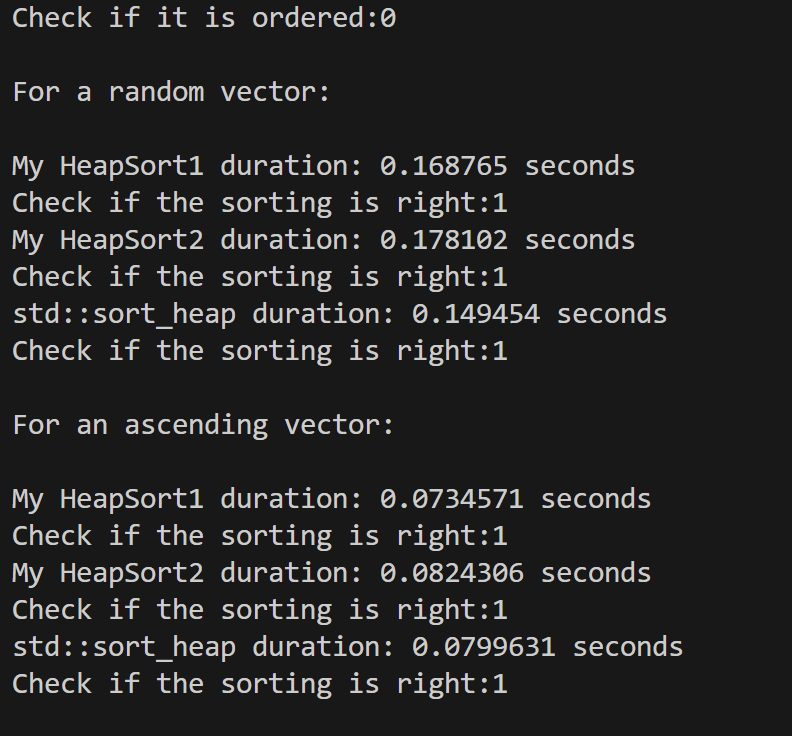
\includegraphics[width=\textwidth]{result1.png}
        \caption{前半部分结果}
        \label{fig:结果1}
    \end{subfigure}
    \hfill
    \begin{subfigure}{0.45\textwidth}
        \centering
        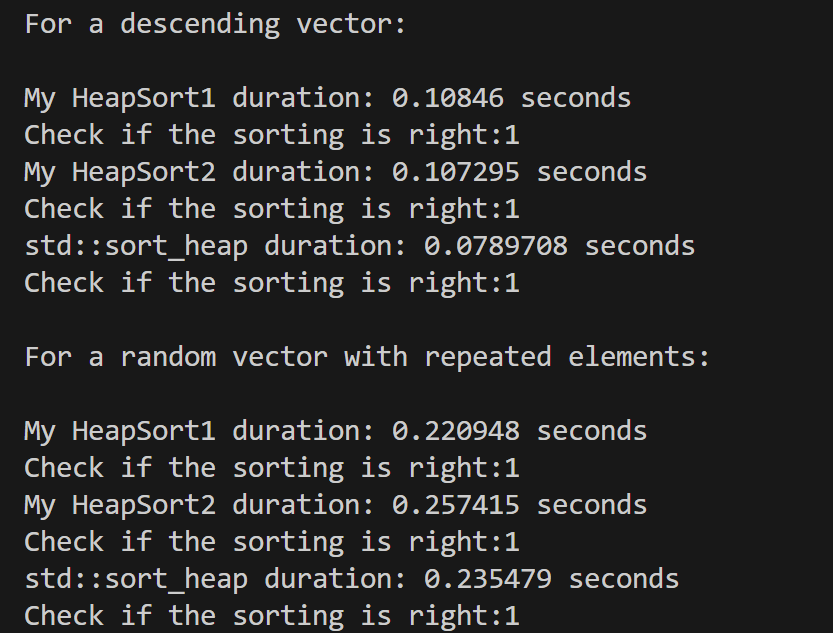
\includegraphics[width=\textwidth]{result2.png}
        \caption{后半部分结果}
        \label{fig:结果2}
    \end{subfigure}
    \caption{测试结果}
    \label{fig:测试结果}
\end{figure}

整理得表格如表\ref{tab:测试结果}所示,表中单位均为s。
\begin{table}[H]
    \centering
    \resizebox{\textwidth}{!}{
    \begin{tabular}{|c|c|c|c|}
        \hline
        \textbf{Vector Type} & \textbf{My HeapSort1 Duration (seconds)} & \textbf{My HeapSort2 Duration (seconds)} & \textbf{std::sort\_heap Duration (seconds)} \\
        \hline
        Random Vector & 0.168765 & 0.178102 & 0.149454 \\
        \hline
        Ascending Vector & 0.0734571 & 0.0824306 & 0.0799631 \\
        \hline
        Descending Vector & 0.10846 & 0.107295 & 0.0789708 \\
        \hline
        Repetitive Vector & 0.220948 & 0.257415 & 0.235479 \\
        \hline
    \end{tabular}
    }
    \caption{效率对比}
    \label{tab:测试结果}
\end{table}

内存泄漏检测,如图\ref{fig:内存泄漏}所示,未发现内存泄漏。利用std内vector,理应自动进行内存管理,不会发生泄漏。
\begin{figure}[H]
    \centering
    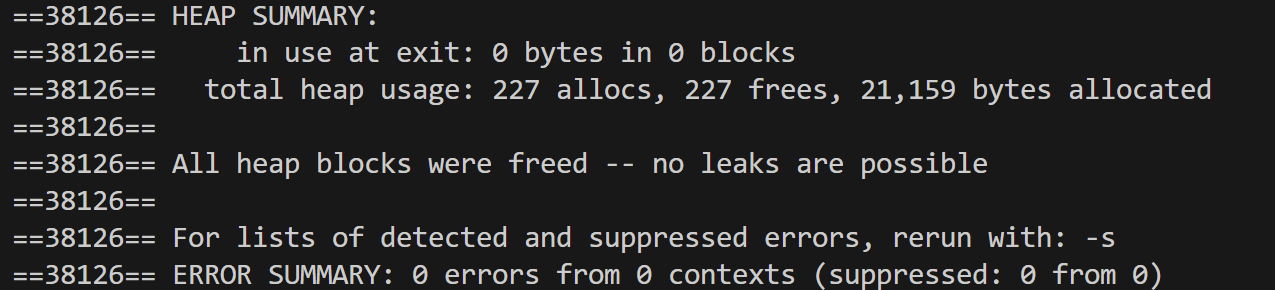
\includegraphics[width=0.6\textwidth]{内存泄漏检查.png}
    \caption{内存泄漏检测}
    \label{fig:内存泄漏}
\end{figure}
\clearpage
\section{结果分析}
由设计思路部分可得,HeapSort1与HeapSort2均为先建堆,建堆操作的时间复杂度为$O(n)$,再逐个取出最小(大)元,取出操作的时间复杂度为$O(\log n)$。
因此总时间复杂度应为$O(n\log n)$。复制、赋值等操作的时间复杂度均为$O(n)$,相比$O(n\log n)$而言为小量,故可忽略。\\
参考表\ref{tab:测试结果}中的结果,\textit{HeapSort1}、\textit{HeapSort2}和\textit{std::sort\_heap}的用时接近,比值在110\% 到 120\%附近。
说明时间复杂度应当在同一阶数,偏差主要可能由自己撰写程序中,一些额外的复制等操作导致,为$O(n)$量级,为可能效率差异原因。\\

\section{心得}
在自建类MyHeap的构建过程中,在各种函数的定义过程中会遇到一些问题,如一些数组的防止越界,下标等计数问题。
起初出现段错误,利用gbd调试,从insert函数到deleteMin函数,经过了多轮调试,并且不断更正。\\
同时,\texttt{test.cpp}文件中的测试函数设计,也不断出错调试,整个过程还是花了很多时间。
最后正确结果出来,实在有点想要泪崩。\\
\end{document}

%%% Local Variables: 
%%% mode: latex
%%% TeX-master: t
%%% End: 
